\chapter{Basismechanismen van een besturingssysteem}

\section{Kernel- en gebruikerstoestand}

Kenmerkend voor het besturingssysteem is dat de programma's, die
er deel van uitmaken, worden uitgevoerd in
\emph{kernel-toestand}\index{kernel mode}\index{supervisor mode} (kernel mode, ook wel supervisor-
of monitor-toestand genoemd). Hiermee duidt men een bijzondere toestand
aan van de processor. Wanneer de processor zich in kernel-toestand
bevindt, beschikt hij over al zijn mogelijkheden. Wanneer de processor
niet in kernel-toestand is, maar in
\emph{gebruikerstoestand} (user mode)\index{user mode}, zijn bepaalde
instructies niet toegelaten.

Tussen de machine-instructies, ingebouwd in de processor, zijn er
namelijk een aantal die men \emph{geprivilegieerde instructies}\index{gepriviligeerde instructie}
noemt. Deze laatste (b.v. instructies voor I/O, voor het
reserveren van geheugenruimte, om de toestand van de processor te
wijzigen enz.) kunnen alleen worden uitgevoerd in kernel-toestand en
zijn daardoor voorbehouden aan het besturingssysteem. De
toepassingssoftware en de overige systeemsoftware worden immers
uitgevoerd in gebruikerstoestand. Wanneer een programma probeert om in
gebruikerstoestand een geprivilegieerde instructie uit te voeren zal een
fatale fout optreden, en het betrokken programma zal be\"eindigd
worden.

Op die manier kunnen allerlei delicate operaties op een
gegarandeerd veilige manier worden uitgevoerd. Ze kunnen namelijk enkel
door het besturingssysteem uitgevoerd worden, waardoor het in staat is
om de omstandigheden waarin deze operaties plaatsvinden volledig te
controleren. Wanneer het besturingssysteem een gewoon programma laat
uitvoeren zal het de processor eerst naar gebruikerstoestand brengen
alvorens het programma te starten (door een sprong). In de
toestandsbeschrijving van de processor is een bit voorzien om de
toestand aan te geven waarin deze zich bevindt: user mode of kernel
mode.

\section{Interrupts}

Een besturingssysteem mag niet worden gezien als een soort
superprogramma, dat voortdurend alle activiteiten in het computersysteem
van boven af regelt. Het komt in tegendeel slechts in actie na een
signaal vanuit de hardware of na een vraag vanuit de toepassingssoftware.
Men zegt dan ook dat een besturingssysteem \emph{gebeurtenisgestuurd},
of \emph{event driven} is.

\begin{figure}
\begin{center}
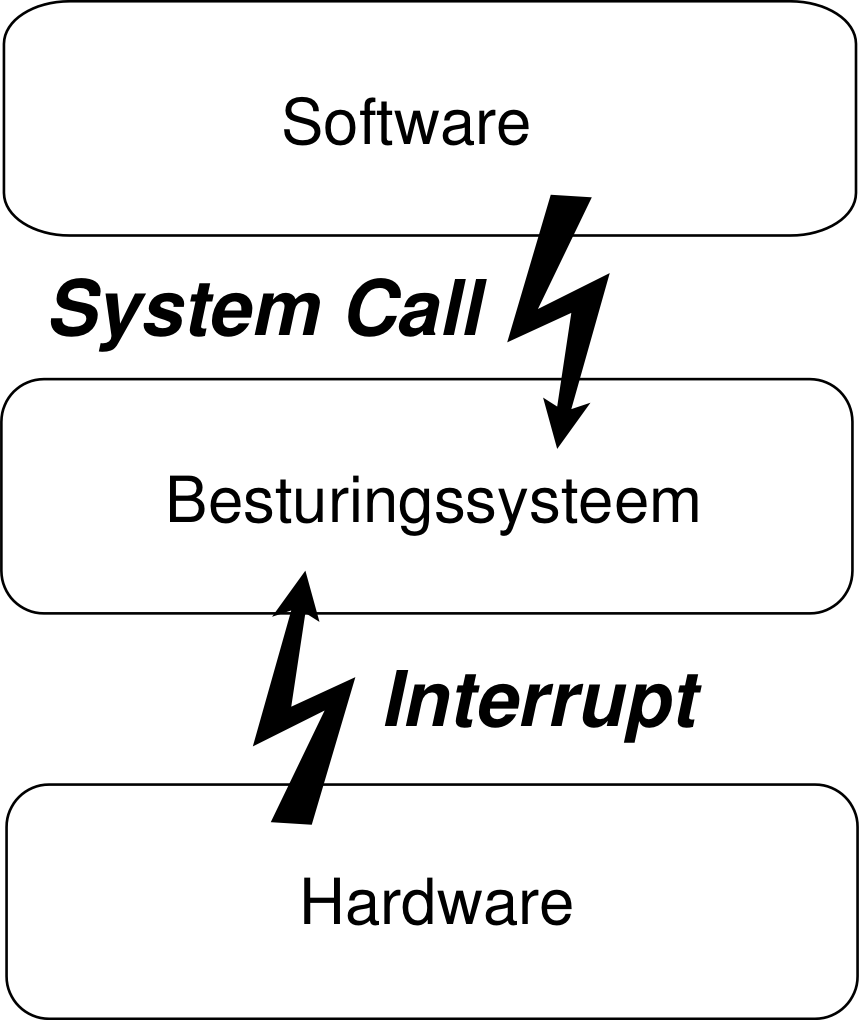
\includegraphics[width=50mm]{images/fig0201.png}
\end{center}
\caption{System calls en interrups}
\label{sysint}
\end{figure}

\subsection{Interrupt requests}

Wanneer vanuit de hardware behoefte is aan een tussenkomst van
het besturingssysteem treedt een \emph{interrupt request}\index{interrupt request} of
\emph{onderbrekingsaanvraag} op. Dit zijn in feite berichtjes die de hardware naar de processor kan sturen wanneer er \emph{iets} gebeurt. De processor ziet dat er een berichtje binnengekomen is, gaat dan de actieve applicatie onderbreken en springt naar code van het besturingssysteem om de interrupt request af te handelen. Wanneer er niets gebeurt komen er geen interrupt requests binnen, en kan de processor volledig gebruikt worden voor het uitvoeren van het actieve programma.

Voor het genereren en afhandelen van interrupt requests is de nodige hardwareondersteuning nodig. Zo moet er bijvoorbeeld bepaald worden wanneer de processor kijkt of er een interrupt request binnengekomen is en hoe die dan afgehandeld moet worden.

In het vak Computersystemen werd uitvoerig uitgelegd hoe de processor instructies verwerkt. Er werd gezegd dat er twee fases zijn: de \emph{haalcyclus} en de \emph{uitvoeringscyclus}. In de haalcyclus werd een bevel opgehaald, en in de uitvoeringscyclus werd het opgehaalde bevel dan uitgevoerd. Na de uitvoeringscyclus gaat de processor terug naar de haalcyclus om het volgende bevel op te halen, enz. Figuur~\ref{fig:nointerrupts} geeft schematisch weer hoe dit proces werkt.

\begin{figure}
  \centering
  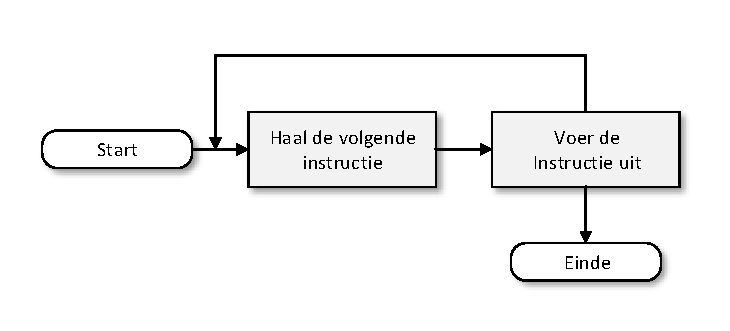
\includegraphics[scale=0.8]{images/NoInterrupts.pdf}
  \caption{Een processor zonder interrupt-ondersteuning.}\label{fig:nointerrupts}
\end{figure}

Wanneer een processor echter het concept van interrupts ondersteunt, wordt het verhaal iets ingewikkelder. Er moet nu namelijk ook regelmatig gecontroleerd worden of er een interrupt request binnengekomen is. Uiteindelijk komen we dan tot het resultaat in figuur~\ref{fig:withinterrupts}. De processor voert nog altijd een haalcyclus en dan een uitvoeringscyclus uit, maar gaat daarna eerst controleren of er een interrupt request binnengekomen is. Indien dit niet het geval is, gaat de processor naar de volgende haalcyclus. Ook indien de afhandeling van interrupt requests (tijdelijk) afgezet is, zal de processor rechtstreeks van de uitvoeringscyclus naar de volgende haalcyclus gaan. In het geval dat er echter wel een interrupt request binnengekomen is, zal de processor de afhandeling van van die interrupt request opstarten (de afhandeling van een interrupt request noemen we \emph{een interrupt}\index{interrupt}).

\begin{figure}
\centering
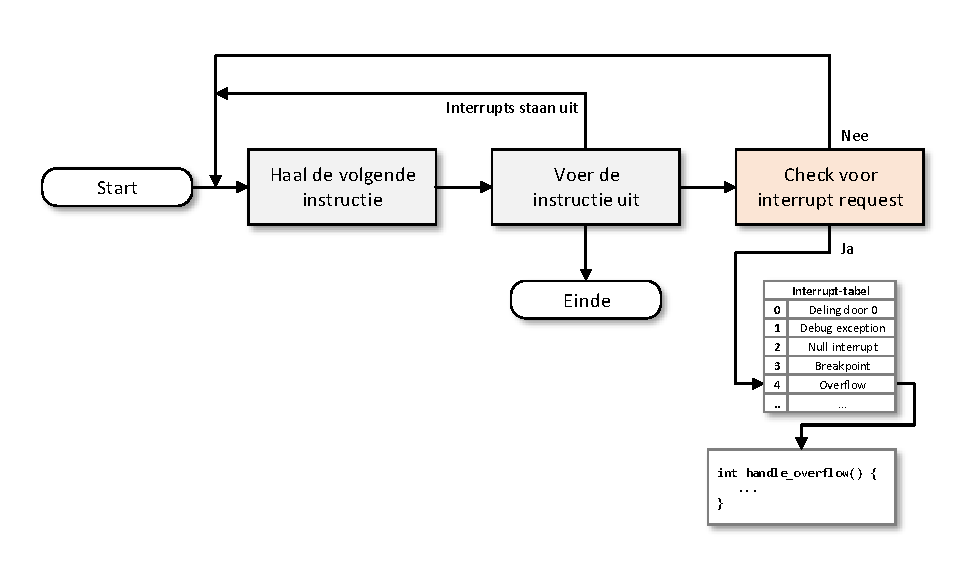
\includegraphics[scale=0.8]{images/WithInterrupts.pdf}
\caption{Een processor met interrupt-ondersteuning.}\label{fig:withinterrupts}
\end{figure}

\subsection{Interrupt requests afhandelen}

Een interrupt request is een elektrisch signaal naar de processor, of
een gebeurtenis binnenin de processor zelf. Als de harde schijf b.v.
een leesopdracht voltooid heeft, zal de schijfbesturingseenheid dit
via een interruptsignaal naar de processor aan het besturingssysteem
melden. Binnen de processor zou een interrupt request kunnen optreden wanneer
een programma deelt door nul, of wanneer een programma een
geprivilegieerde (en dus niet toegelaten) instructie gebruikt.

Deze verschillende types van interrupts moeten allemaal op andere manieren behandeld worden. Om het een en ander te vereenvoudigen bestaat er een \emph{interrupttabel}\index{interrupttabel} die voor elk type interrupt een geheugenadres van een methode bijhoudt die opgeroepen moet worden wanneer een overeenkomstige interrupt request binnenkomt.

Op de Intel x86-processor bestaat de interrupttabel uit 256 waardes (ook wel \emph{interrupt vectors} genoemd). De eerste 32 waardes zijn gereserveerd voor Intel en worden gebruikt om processorfouten af te handelen. De overige waardes kunnen ingesteld worden door het besturingssysteem, afhankelijk van de hardware die aanwezig is in het systeem. Als er bijvoorbeeld een netwerkkaart aanwezig is, kan het besturingssysteem bijvoorbeeld het interrupt nummer 97 toekennen aan die kaart (eender welk vrij nummer kan natuurlijk gekozen worden). Wanneer die netwerkkaart dan een netwerkpakketje binnenkrijgt, moet het een interrupt request met waarde 97 sturen naar de processor. Zo weet het besturingssysteem dat de interrupt van de netwerkkaart komt. Een overzicht vind je in figuur~\ref{table:ivt}.

\begin{figure}
\centering
\begin{tabular}{|c|l|}
  \hline
  \textbf{Interrupt nummer} & \textbf{Beschrijving (Engels)} \\
  \hline
  0 & divide error \\
  1 & debug exception \\
  2 & null interrupt \\
  3 & breakpoint \\
  4 & overflow \\
  5 & bound range exception \\
  6 & invalid processor instruction \\
  7 & device not available \\
  8 & double fault \\
  9 & coprocessor segment overrun \\
  10 & invalid task state segment \\
  11 & segment not present \\
  12 & stack fault \\
  13 & general protection \\
  14 & page fault \\
  15 & (Intel reserved, do not use) \\
  16 & floating-point error \\
  17 & alignment check \\
  18 & machine check \\
  19-31 & (Intel reserved, do not use) \\
  32-255 & maskable interrupts \\
  \hline
\end{tabular}
\caption{De inhoud van de Intel x86 interrupttabel.}
\label{table:ivt}
\end{figure}

Wanneer er een interrupt binnenkomt, gaat de processor de juiste entry van de interrupttabel opvragen en daar naartoe springen. Figuur~\ref{fig:withinterrupts} toont bijvoorbeeld de afhandeling van een overflowfout (d.i. interrupttype 4). Wanneer die fout zich voordoet gaat de processor in de interrupttabel de interrupt vector op plaats 4 opvragen. Deze verwijst dan door naar de methode \emph{handle\_overflow} die een deel is van het besturingssysteem en de fout afhandelt. Zulke methodes noemen we ook wel \emph{interrupt service routines}.

Laten we het voorbeeld van de leesopdracht voor de harde schijf
even bekijken (figuur \ref{lezenhd}).

\begin{figure}
\begin{center}
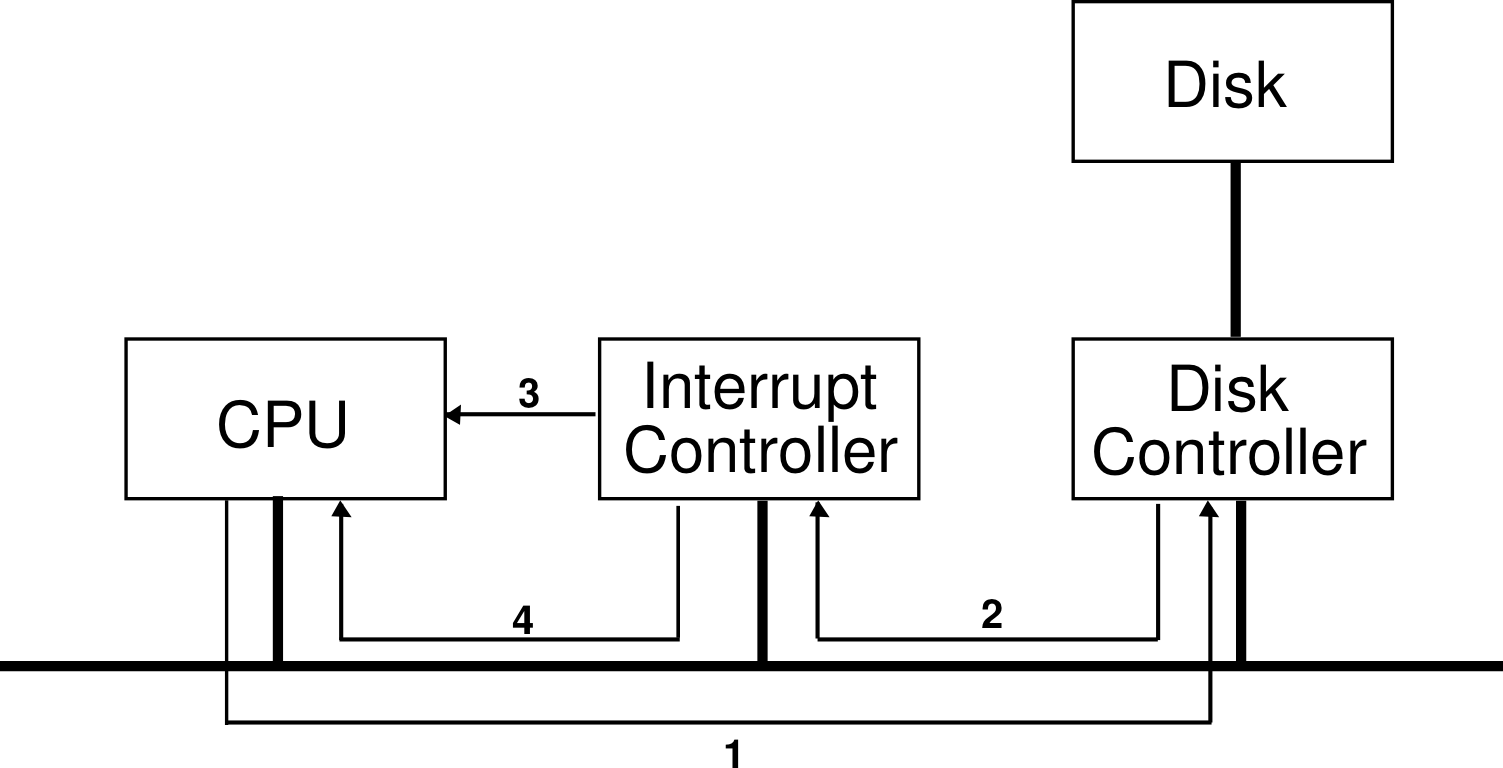
\includegraphics[width=80mm]{images/fig0202.png}
\end{center}
\caption{Lezen van een harde schijf}
\label{lezenhd}
\end{figure}

\begin{enumerate}
\item Schijfbesturingseenheid ontvangt een leesopdracht.
\item Wanneer de leesopdracht voltooid is stuurt de schijfbesturingseenheid een
interrupt request naar de \emph{interrupt controller}. Merk op dat de
processor tussen 1 en 2 \'e\'en of meer andere programma's heeft uitgevoerd.
\item De interrupt controller geeft de interrupt request door aan de processor. Wanneer
er een request met een hogere prioriteit wordt afgehandeld is het mogelijk dat
de schijf-interrupt hierop moet wachten. Dit is \'e\'en van de taken van de
interrupt controller.
\item Interrupt controller stuurt het volgnummer van de bron van de interrupt request
naar de processor, zodat die weet welk apparaat de request veroorzaakte.
\item De processor zoekt het adres op van de juiste Interrupt Handler in de
tabel met interrupt-vectoren.
\item De inhoud van de bevelenteller, alle registers en de processorstatus
worden op de stapel gezet.
\item Adres van Interrupt Handler wordt in bevelenteller geplaatst en de
processor wisselt naar kernel toestand.
\item Sprong naar het adres van de Interrupt Handler en de handler wordt
uitgevoerd. De code in de interrupt handler handelt het via de interrupt gedane
verzoek af. Deze handler is een onderdeel van het besturingssysteem, en een
gedeelte van de code zal uit de device driver van het onderbrekende apparaat
komen.
\item Als het werk erop zit herstelt de interrupt handler de bevelenteller,
registers en processortoestand en schakelt de processor terug in
gebruikerstoestand. Het programma dat in uitvoering was voor de interrupt wordt
verdergezet (want de bevelenteller wijst naar de volgende instructie in dat
programma).
\end{enumerate}

Het gevolg van een interrupt is dus dat een stuk code van het
besturingssysteem uitgevoerd wordt, dat specifiek bestemd is om de
opgetreden interrupt af te handelen, de Interrupt Handler. Deze zal
eerst nagaan wat de reden is van de interrupt en zal dan de gepaste
acties ondernemen.

Stappen 6 en 7 worden een \emph{context switch}\index{context switch}
genoemd. Een context switch wijzigt de toestand van de processor zodat
die een ander programma gaat uitvoeren, en bovendien zo dat de
toestand weer hersteld kan worden om verder te gaan met de uitvoering
van het programma dat in uitvoering was. De inhoud van de
bevelenteller, de registers en het statuswoord van de processor worden
weggeschreven op de stapel in het werkgeheugen. Deze gegevens worden
de context genoemd, vandaar de term context switch.

Merk op dat dit door de processor zelf afgehandeld wordt, en
niet door een stukje machine-code uit te voeren. Om dit stukje code
voor de context switch uit te voeren zou immers een context switch
nodig zijn...

\subsection{Snelheidswinst}

Nu dat we het concept van interrupts ge\"introduceerd hebben, kunnen we deze aanpak vergelijken met de standaard-aanpak waarbij er geen interrupts gebruikt worden. Figuur~\ref{fig:intsandnoints} toont de uitvoering van een programma zonder interrupts, en hetzelfde programma m\'et interrupts. Voor schema~\ref{fig:progflownoint} doorloopt het progamma de volgende stappen:

\begin{enumerate}
\item Het programma doet een berekening. Het wil uiteindelijk de resultaten wegschrijven naar de schijf, dus verstuurt het een aanvraag naar het besturingssysteem om de data weg te schrijven. Het programma zelf kan dit natuurlijk niet, aangezien het geen rechten heeft om rechtstreeks de hardware aan te spreken.
\item Het besturingssysteem evalueert de aanvraag en wanneer alles ok is stuurt het de data naar de schijf om deze weg te schrijven.
\item De schijf schrijft de data weg. De processor doet ondertussen niet veel nuttigs: hij blijft in een lus aan de schijf vragen of die al klaar is.
\item Uiteindelijk geeft de schijf aan dat het wegschrijven gedaan is, en sluit het besturingssysteem de schrijfopdracht af. Hierna gaat de processor terug naar de applicatie.
\item De applicatie gaat verder en sluit uiteindelijk af.
\end{enumerate}

Schema~\ref{fig:progflowwithint} toont de uitvoering van hetzelfde programma m\'et interrupts. Het doorloopt de volgende stappen:

\begin{enumerate}
\item Het programma doet een berekening. Het wil uiteindelijk de resultaten wegschrijven naar de schijf, dus verstuurt het een aanvraag naar het besturingssysteem om de data weg te schrijven.
\item Het besturingssysteem evalueert de aanvraag en wanneer alles ok is stuurt het de data naar de schijf om deze weg te schrijven.
\item De schijf schrijft de data weg. De processor gaat ondertussen terug naar de applicatie die verder kan rekenen terwijl de schijf data schrijft. De applicatie blijft actief totdat de schijf klaar is en een interrupt request stuurt.
\item De interrupt request wordt afgehandeld (d.i. een interrupt) en het besturingssysteem sluit de schrijfopdracht af. Hierna gaat de processor terug naar de applicatie.
\item De applicatie gaat verder en sluit uiteindelijk af.
\end{enumerate}

\begin{figure}
\centering
\begin{subfigure}{.5\textwidth}
  \centering
  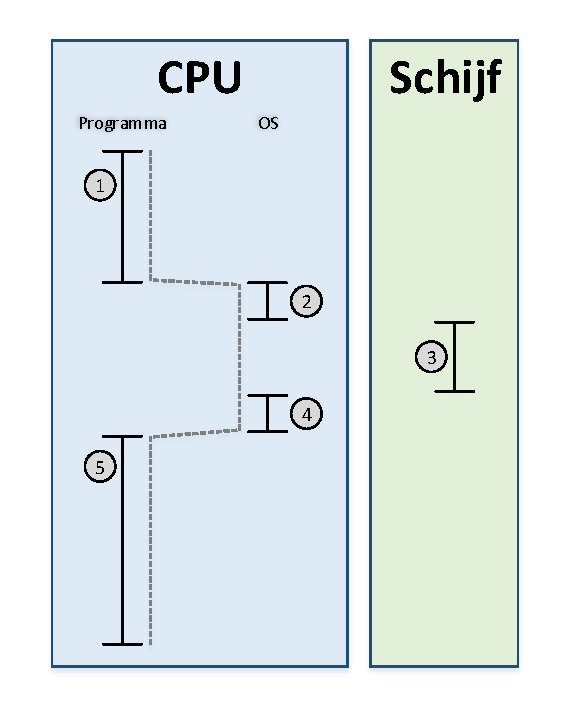
\includegraphics[width=.85\linewidth]{images/ProgramFlowNoInterrupts.pdf}
  \caption{Geen interrupts}
  \label{fig:progflownoint}
\end{subfigure}%
\begin{subfigure}{.5\textwidth}
  \centering
  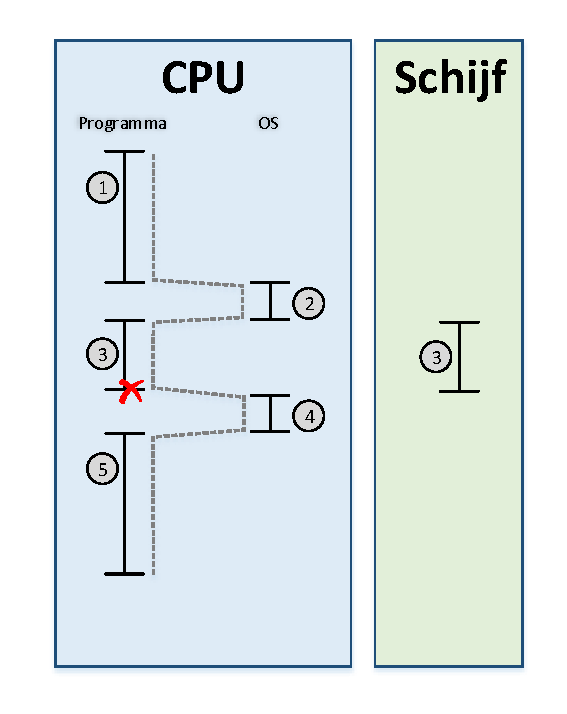
\includegraphics[width=.85\linewidth]{images/ProgramFlowWithInterrupts.pdf}
  \caption{Wel interrupts}
  \label{fig:progflowwithint}
\end{subfigure}
\caption{De uitvoering van een programma met en zonder interrupts.}
\label{fig:intsandnoints}
\end{figure}

Merk op dat het proces in schema~\ref{fig:progflowwithint} een aanzienlijke tijdswinst boekt, aangezien het tijdens het wegschrijven van data nog altijd kan blijven doorrekenen. Hier wordt het voordeel van interrupts dan ook duidelijk.

\subsection{Soorten interrupts}

Er zijn twee soorten interrupts: externe en interne.
\emph{Externe interrupts} komen van hardware buiten de
processor. Enkele voorbeelden:

\begin{description}
\item[Klok interrupts] De interne klok van de computer signaleert hiermee aan de
processor dat een bepaalde tijdsperiode is verstreken.
\item[I/O interrupts] Wanneer via een randapparaat een I/O operatie is
uitgevoerd meldt de besturingseenheid die het randapparaat
bestuurt, op deze manier het einde van de I/O operatie (zoals in het voorbeeld
hierboven)
\item[Keyboard interrupts] Telkens wanneer een toets op het toetsenbordwordt
ingedrukt heeft dit een interrupt tot gevolg, die tot doel heeft het
overeenstemmende karakter te laten inlezen in een buffer zodat het programma
waarvoor de invoer bestemd is eraan
kan.
\item[Hardwarefouten] Wanneer de hardware een fout detecteert, zoals bijvoorbeeld
 een printer die een papierstoring detecteert, wordt er een interrupt request gegenereerd.
\end{description}

\emph{Interne interrupts} worden veroorzaakt
door een gebeurtenis binnen de processor en kunnen nog eens worden
opgesplitst in twee groepen: uitzonderingen en software
interrupts.

\emph{Uitzonderingen} of \emph{exceptions} zijn het gevolg van een fout tijdens
de uitvoering van een instructie zoals het delen van een getal door
nul, het adresseren van een ongeldig adres in het geheugen of een
poging om in gebruikerstoestand een geprivilegieerde instructie uit te
voeren. Het besturingssysteem moet hier optreden, b.v. door het
overtredende programma af te sluiten en dit aan de gebruiker mee te
delen. Uitzonderingen die door het besturingssysteem kunnen hersteld worden noemen we we in
het Engels \emph{faults}. Zo valt een deling door nul onder de noemer 'faults', omdat het besturingssysteem die situatie kan corrigeren door bijvoorbeeld een exception in het desbetreffende programma te gooien. Andere uitzonderingen die niet hersteld kunnen worden, noemen we \emph{aborts}. Een abort kan je bijvoorbeeld krijgen wanneer er een deling door nul optreedt tijdens de uitvoering van een interruptroutine.

\emph{Traps} of \emph{software interrupts} zijn het gevolg van de uitvoering van speciaal
daarvoor voorziene instructies in een programma. Zo kunnen programma's
ook gebruik maken van de mogelijkheden van het interrupt mechanisme en
de hulp inroepen van het besturingssysteem. Als een programma b.v.
gegevens wil inlezen vanop de schijf zal het dit via een software
interrupt aan het besturingssysteem vragen. In Intel x86 assembler wordt de INT-instructie gebruikt om een
software interrupt aan te geven. Met deze instructie kan een getal
tussen 0 en 255 meegegeven worden.

Er is een subtiel verschil tussen de verschillende interrupt types: interne interrupts zijn
\emph{synchroon}, terwijl externe interrupts \emph{asynchroon} zijn.

Bij synchrone interrupts gebeurt de afhandeling ``actief'' in die zin dat de code van de
actieve applicatie verwacht dat de interrupts afgehandeld worden en hier zelfs op steunt.

Asynchrone interrupts gebeuren niet op voorspelbare plaatsen in de applicatiecode. Ze zijn
``passief'' omdat de interrupt handlers gewoon wachten totdat de interrupt requests
uiteindelijk eens voorkomen. Ze zijn ook onafhankelijk van en ongerelateerd met de actieve applicatie.

Op de Intel x86 processor kunnen asynchrone interrupts gemaskeerd worden. Dat wil zeggen
dat er tijdelijk gekozen kan worden om die interrupts niet af te handelen. Synchrone
interrupts kunnen nooit gemaskeerd worden, maar aangezien deze enkel gegenereerd worden
door het actieve programma (en volledig afgehandeld worden eer het programma terug verder mag
gaan) gaat de ene synchrone interrupt normaal nooit een andere onderbreken. Soms kan dit 
echter toch het geval zijn wanneer er een fout zit in het besturingssysteem. Vaak resulteert
dit in een crash van het besturingssysteem\footnote{Op Windows krijg je dan het alom bekende 
\emph{blue screen of death}. Volgens Microsoft zijn ongeveer 25\% van de blue screens veroorzaakt
door een echte fout in de code van Windows, terwijl de overige 75\% veroorzaakt worden door drivers
van externe partijen.}.

\subsection{Interrupts identificeren}

Hoe wordt nu bepaald welke interrupt handler dient te worden
uitgevoerd wanneer een interrupt optreedt? Bij exceptions wordt de
interrupt door de processor zelf veroorzaakt, en kan de processor de
inhoud van de conditiecode in zijn toestandsbeschrijving
nagaan.

Wanneer een programma in uitvoering een trap-instructie doet
wordt de nodige informatie meegegeven om de juiste interrupt handler
te kiezen. In Intel x86 assembler is dit het getal dat je meegeeft aan de
INT-instructie. Natuurlijk hangt de betekenis van het getal af van het
gebruikte besturingssysteem.

In Intel x86 assembler programma's voor MS-DOS wordt vaak 'INT 21h'
opgeroepen. Deze software interrupt zorgt ervoor dat MS-DOS een
interrupt handler uitvoert. Deze specifieke interrupt handler is een
soort manusje-van-alles in MS-DOS, en je moet via het AH-register
aangeven wat je van de interrupt handler verwacht. Als er b.v. '4Ch'
in AH staat moet het besturingssysteem je programma be\"eindigen.

Bij hardware interrupts ligt de oorzaak buiten de processor, en
moeten we op zoek naar de bron van de onderbreking. Dat kan op 3
algemene manieren.

\begin{figure}
\begin{center}
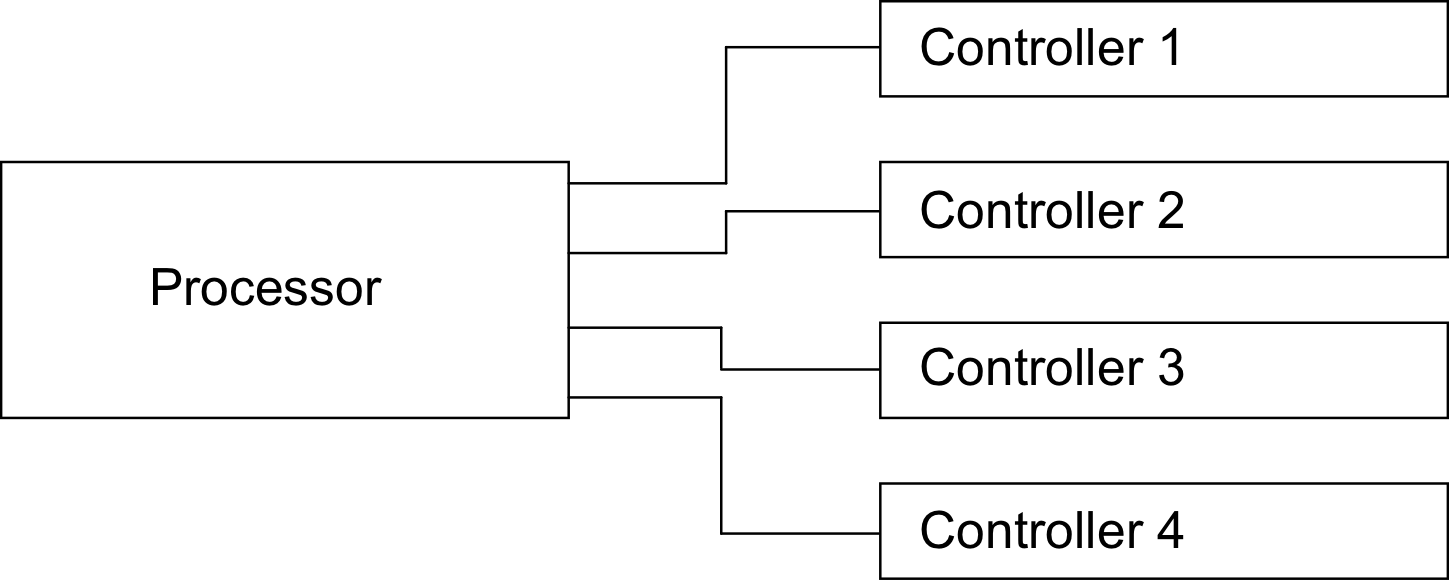
\includegraphics[width=80mm]{images/fig0203.png}
\end{center}
\caption{Controllers met eigen interruptlijnen}
\label{eigenlijn}
\end{figure}

Als iedere controller een eigen
\emph{interruptlijn}\index{interruptlijn} heeft, bepaalt de lijn waarop het
interruptsignaal verschijnt meteen welke handler moet worden
uitgevoerd (figuur \ref{eigenlijn}). Dit is een snelle en eenvoudige methode
maar legt
natuurlijk zware beperkingen op aan de configuratiemogelijkheden: het
aantal controllers is dan beperkt tot het aantal interruptlijnen in de
processor.

\begin{figure}
\begin{center}
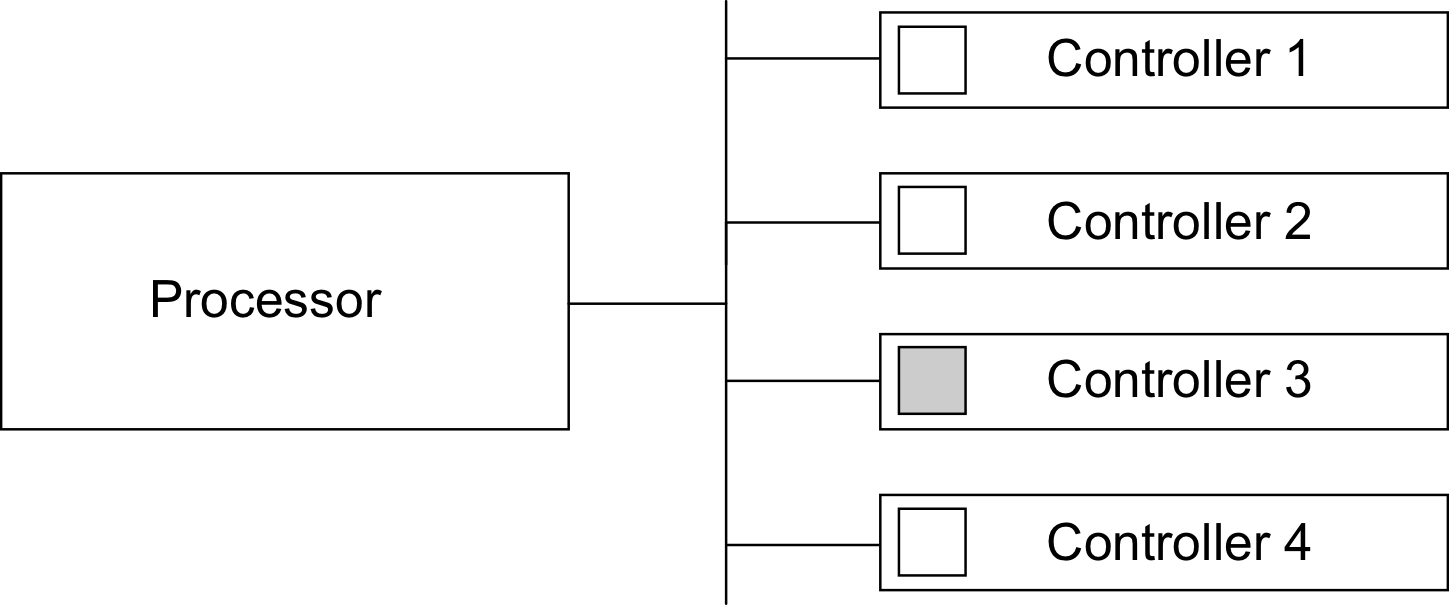
\includegraphics[width=80mm]{images/fig0204.png}
\end{center}
\caption{Software Polling}
\label{eenlijn}
\end{figure}

Als de controllers via \'e\'en lijn met de processor verbonden zijn
kan de controller d.m.v. een bit in \'e\'en van zijn registers aangeven of
hij een interrupt heeft gestuurd of niet. Na de context switch wordt
een routine uitgevoerd die aan \emph{software polling}
doet: achtereenvolgens elke controller controleren tot diegene wordt
gevonden die de interrupt veroorzaakte. Door het uitvoeren van deze
extra routine is dit een eerder trage methode.

\begin{figure}
\begin{center}
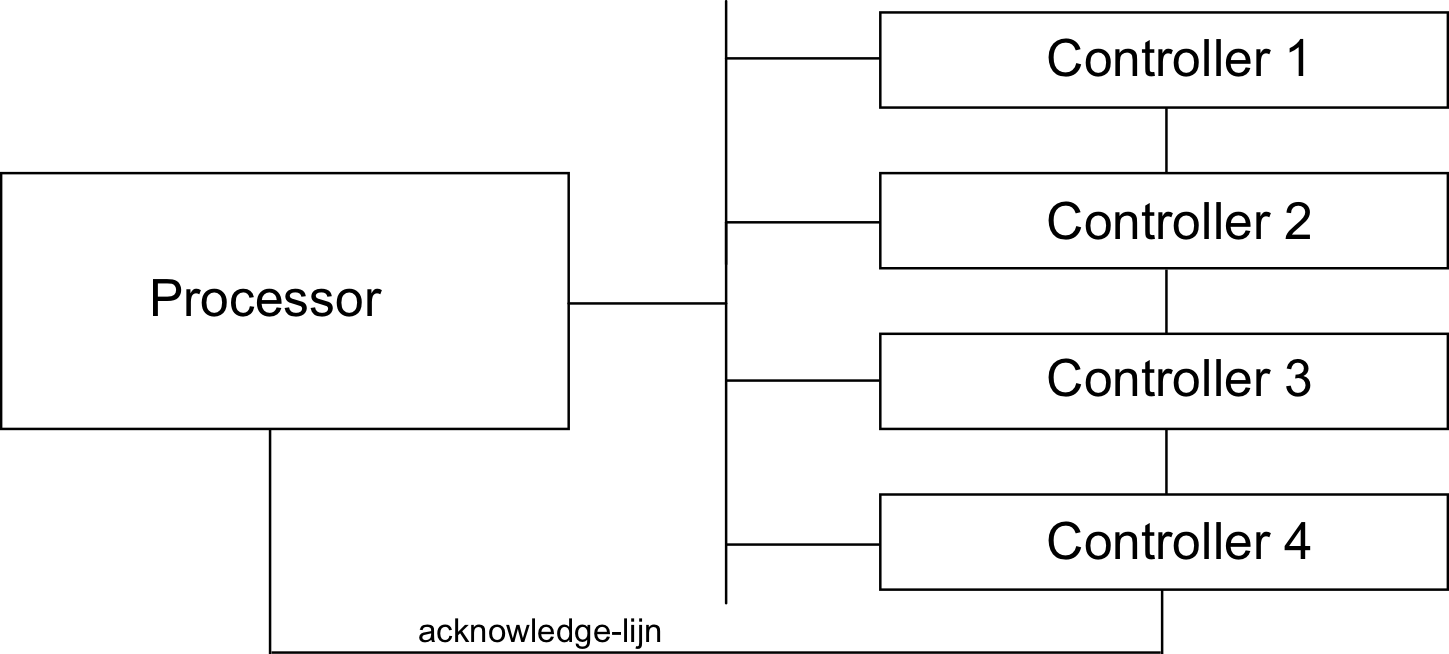
\includegraphics[width=80mm]{images/fig0205.png}
\end{center}
\caption{Daisy Chaining}
\label{daisy}
\end{figure}

Bij de derde manier zijn alle controllers via \'e\'en interruptlijn
en \'e\'en zogenaamde acknowledge-lijn met de processor verbonden. Zodra
een hardware interrupt optreedt zendt de processor via deze
acknowledge-lijn een signaal naar de eerste controller. Indien deze de
interrupt veroorzaakte stuurt hij een identificatiecode naar de
processor; in het andere geval geeft hij het signaal door naar de
volgende controller, die hierop op dezelfde manier reageert. Deze
werkwijze, \emph{daisy chaining}\footnote{In het algemeen is daisy chaining een
structuur waarin een apparaat A verbonden is met een apparaat B, B met C, C met
D, enz. Als A een signaal ontvangt stuurt hij het door naar B, eventueel na het
aanbrengen van een wijziging. De naam komt van het vormen van een slinger van
madeliefjes (Eng.: daisy) door een gaatje te maken in de stengel van een bloem
en er een andere bloem door te steken. Een ander voorbeeld van het gebruik van
een daisy chain structuur zijn SCSI-apparaten.}\index{daisy chaining} genoemd, is erg snel omdat ze
volledig via de hardware verloopt.

\subsection{Prioriteiten voor interrupts}

Het is soms belangrijk dat bepaalde interrupts voorrang krijgen
krijgen op minder belangrijke. De volgorde waarin interrupts worden
afgehandeld verdient dus ook aandacht.

Wanneer twee of meer interrupts tegelijk (of juister: tijdens
het uitvoeren van dezelfde instructie) optreden, moet er gekozen
worden welke interrupt eerst afgehandeld wordt. Beide interrupts zijn
hangende of pending. Vaak wordt gekeken naar de vereiste
\emph{interrupt latency}. Dit is de maximale tijd die
waarbinnen de interrrupt afhandeling moet begonnen zijn. De drivers
van audio- of video-hardware hebben een lage interrupt latency. Als
het te lang duurt vooraleer hun interrupts behandeld worden ontstaat
er kwaliteitsverlies.

Hoe we de prioriteit van interrupts kunnen bepalen hangt af van
de gebruikte identificatiemethode. Bij het gebruik van meerdere
interruptlijnen zal de processor zelf moeten beslissen aan welk
signaal hij eerst aandacht zal besteden. Bij software polling zal de
volgorde waarin de controllers worden nagekeken bepalend zijn voor de
prioriteit. Dit kan softwarematig worden ingesteld. Bij daisy chaining
is het de volgorde waarin de controllers worden aangesloten op de
acknowledge-lijn. Een duidelijk nadeel is hier dat een wijziging in de
prioriteit een ingreep in de hardware vereist.

Een tweede vraag die we ons moeten stellen is of we nieuwe
interrupts willen toelaten tijdens het afhandelen van een interrupt.
Vaak wordt een vlag voorzien waarmee alle interrupts tijdelijk
geblokkeerd worden. Andere systemen laten toe prioriteiten te
defini\"eren voor de interrupts, en tijdens de afhandeling van een
bepaalde interrupt worden alleen interrupts geaccepteerd met een
hogere prioriteit.

\section{System Calls}\label{systemcalls}

Interrupts vormen de schakel tussen het besturingssysteem en de
hardware. \emph{System calls}\index{system calls} of
\emph{systeemaanroepen} leggen een link tussen de
overige software en het besturingssysteem (zie figuur \ref{sysint}). Bij alle
activiteiten, uitgevoerd in gebruikerstoestand, is immers zeer frequent de
tussenkomst nodig van het besturingssysteem om operaties te kunnen uitvoeren die
alleen in kernel-toestand mogelijk zijn.

\subsection{Het uitvoeren van een system call}

Essentieel bij een system call is het overschakelen van de
processor naar kernel- toestand. Dit gebeurt altijd via een
trap-instructie (software-interrupt)\index{trap}, waardoor wordt vermeden dat na
het instellen van de kernel-toestand het gebruikersprogramma de
controle zou kunnen behouden. De trap-instructie zorgt er namelijk
voor dat de gepaste systeemroutine wordt gestart. Daartoe wordt als
operand voor de trap-instructie een code meegegeven. Extra informatie kan
eventueel in welbepaalde registers worden geplaatst.

Figuur~\ref{fig:systemcalls} toont hoe een programma zichzelf kan afsluiten door
de juiste software interrupt op te roepen. Op Intel x86 wordt de \texttt{int}-instructie
als trap-instructie gebruikt, terwijl op een ARM-processor de \texttt{swi}-instructie
gebruikt wordt. Afhankelijk van de operanden van deze instructie en de waardes in de registers
weet het besturingssysteem wat de applicatie wil doen.

\begin{figure}
  \centering
  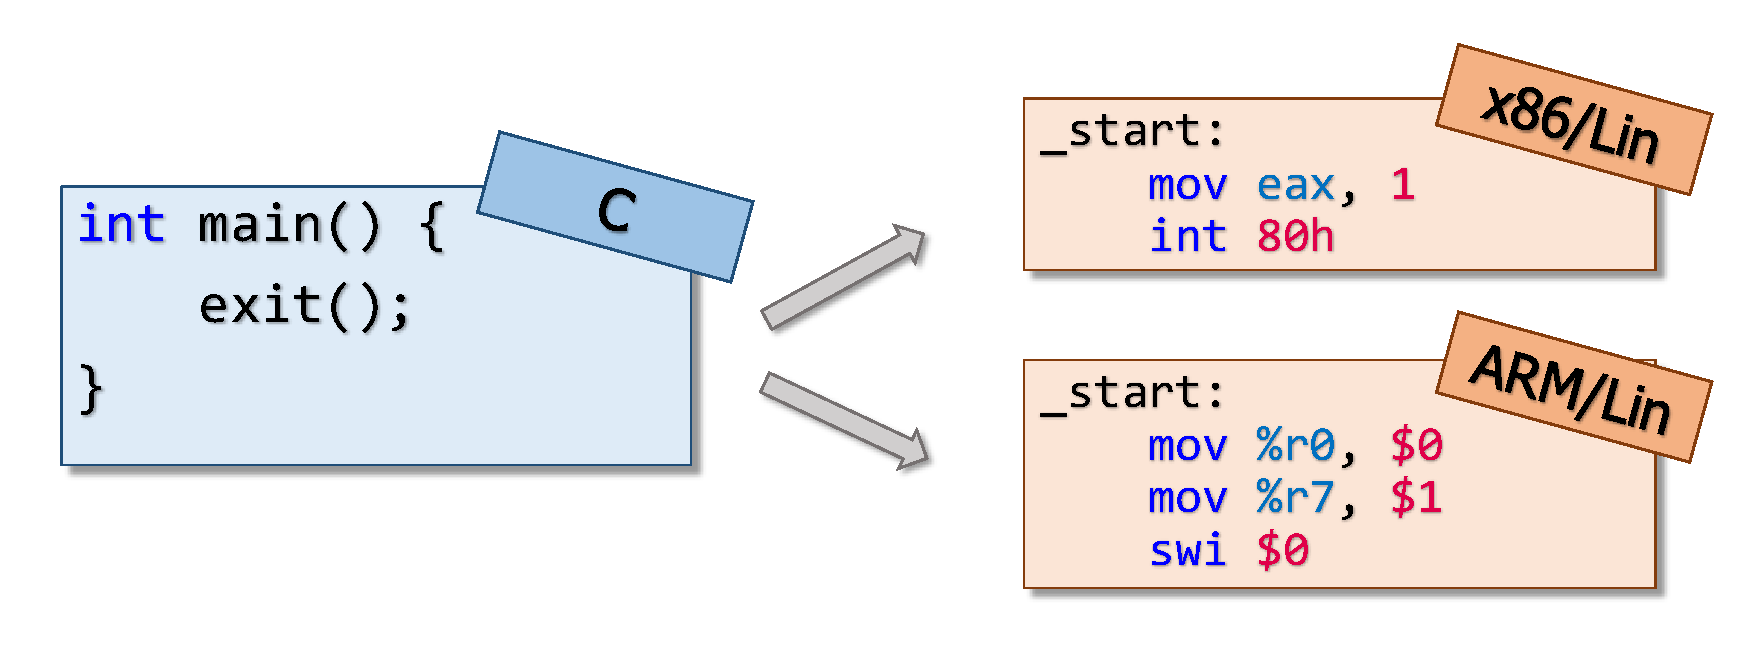
\includegraphics[scale=0.4]{images/IntInstructions.pdf}
  \caption{Het gebruik van traps om system calls uit te voeren.}\label{fig:systemcalls}
\end{figure}

Omdat de trap functioneert als een interrupt zal een interrupt
handler worden opgestart in kernel mode, die de meegegeven code zal
vertalen naar het beginadres van een specifieke systeemroutine. Aan de
hand van de code wordt tevens bepaald hoeveel bytes aan informatie als
parameters aan de systeemroutine moeten worden doorgegeven. Deze bytes
worden dan klaargezet, waarna de systeemroutine kan worden
opgeroepen.

Zodra de opdracht voltooid is wordt een eventueel resultaat (of
een foutmelding) op een afgesproken plaats gedeponeerd, waarna de
processor wordt teruggeschakeld naar user mode en tenslotte wordt
teruggekeerd naar het oproepend programma.

\subsection{Beschikbare system calls}

Dit is een overzicht van typische taken die toepassingssoftware
via system calls door het besturingssysteem kan laten
uitvoeren:

\begin{itemize}
\item Opstarten en be\"eindigen van programma's.
\item Laten wachten van een programma op een gebeurtenis.
\item Toekennen en vrijgeven van geheugen.
\item Bestandsbeheer.
  \begin{itemize}
  \item Cre\"eren en vernietigen van bestanden en directories.
  \item Openen en sluiten van bestanden.
  \item Lezen en schrijven in bestanden.
  \item Bepalen van de toegang tot bestanden.
  \end{itemize}
\item Besturing en beheer van randapparaten.
  \begin{itemize}
  \item Verwerven en afstaan van een randapparaat.
  \item Positioneren van een randapparaat.
  \item Lezen van en schrijven naar een randapparaat.
  \item Opnemen in of verwijderen uit de configuratie.
  \end{itemize}
\item Uitwisselen van informatie.
  \begin{itemize}
  \item Opvragen of wijzigen van informatie over:
    \begin{itemize}
    \item systeemconfiguratie
    \item uitgevoerde activiteiten
    \item processen
    \item bestanden en directories
    \item gebruikers
    \end{itemize}
  \end{itemize}
\item Communicatie
  \begin{itemize}
  \item Cre\"eren en opheffen van verbindingen (tussen systemen en processen)
  \item Zenden en ontvangen van boodschappen (tussen systemen, processen en
gebruikers)
  \end{itemize}
\end{itemize}

\subsection{Voorbeeld}

In het volgende voorbeeld simuleren we een oproep van de
read-system call in Linux. Deze kan in de programmeertaal C opgeroepen
worden d.m.v. de functie \texttt{read(file\_desc, buffer, nbytes)}. Wanneer een
programma deze functie aanroept zal het volgende gebeuren:

\begin{enumerate}
\item Oproepend programma zet de waarden van de drie parameters op de stapel.
\item Read functie wordt aangeroepen (sprong naar code van read-functie).
\item Functie zet system call nummer in het juiste register en voert
TRAP-instructie uit (in Linux op een Intel x86 processor zou dit de instructies \texttt{mov eax, 3}
en \texttt{int 80h} opleveren; de 3 in eax geeft aan dat het om een lees-operatie gaat).
\item Besturingssysteem zoekt juiste routine op voor de system call.
\item BS start systeemroutine (sprong).
\item Systeemroutine zet resultaat op voorziene plaats, verlaat kernel mode en
geeft controle terug aan read-functie.
\item Read functie ontvangt de gegevens, zet ze op hun plaats en geeft controle
terug aan oproepend programma's.
\item Uitvoer oproepend programma gaat verder.
\end{enumerate}

Stappen 4 t/m 6 verlopen in kernel mode, de overige stappen worden in user mode
uitgevoerd.

